\documentclass[12pt,titlepage]{article}
\usepackage[margin=1.25in]{geometry}
\usepackage{graphicx,amsmath,blindtext,minted}

%% Variables definition
\newcommand{\vSubject}{Advanced Web Programming}
\newcommand{\vSubtitle}{Model and Eloquent Orm}
\newcommand{\vName}{Muhammad Baihaqi Aulia Asy'ari}
\newcommand{\vNIM}{2241720145}
\newcommand{\vClass}{2I}
\newcommand{\vDepartment}{Information Technology}
\newcommand{\vStudyProgram}{D4 Informatics Engineering}

%% [START] Tikz related stuff
\usepackage{tikz}
\usetikzlibrary{svg.path,calc,shapes.geometric,shapes.misc}
\tikzstyle{terminator} = [rectangle, draw, text centered, rounded corners = 1em, minimum height=2em]
\tikzstyle{preparation} = [chamfered rectangle, chamfered rectangle sep=0.75em, draw, text centered, minimum height = 2em]
\tikzstyle{process} = [rectangle, draw, text centered, minimum height=2em]
\tikzstyle{decision} = [diamond, aspect=2, draw, text centered, minimum height=2em]
\tikzstyle{data}=[trapezium, draw, text centered, trapezium left angle=60, trapezium right angle=120, minimum height=2em]
\tikzstyle{connector} = [line width=0.25mm,->]
%% [END] Tikz related stuff

%% [START] Fancy header related stuff
\usepackage{fancyhdr}
\pagestyle{fancy}
\setlength{\headheight}{15pt} % compensate fancyhdr style
\fancyhead{}
\fancyfoot{}
\fancyfoot[L]{\thepage}
\fancyfoot[R]{\textit{\vSubject - \vSubtitle}}
\renewcommand{\footrulewidth}{0.4pt}% default is 0pt, overline for footer
%% [END] Fancy header related stuff

%% [START] Custom tabular command related stuff
\usepackage{tabularx}
\newcommand{\details}[2]{
    #1 & #2  \\
}
%% [END] Custom tabular command related stuff

%% [START] Figure related stuff
\newcommand{\image}[3][1]{
    \begin{figure}[h]
        \centering
        \includegraphics[#1]{#2}
        \caption{#3}
        \label{#3}
    \end{figure}
}
%% [END] Figure related stuff

%%
\usepackage{pgf-umlcd}

\renewcommand{\umldrawcolor}{black}
\renewcommand{\umlfillcolor}{white}
%%

%% [BEGIN] Custom enumerator
\usepackage{enumitem}
%% [END] Custom enumerator

%% [BEGIN] Paragraph indent
\usepackage{indentfirst}
%% [END] Paragraph indent

%% [BEGIN] URL
\usepackage{hyperref}
\hypersetup{
    colorlinks=true,
    linkcolor=blue,
    filecolor=magenta,      
    urlcolor=cyan,
    pdftitle={Overleaf Example},
    pdfpagemode=FullScreen,
    }

\urlstyle{same}
%% [END] URL

\begin{document}
\begin{titlepage}
    \centering
    \vfill
    {\bfseries\LARGE
        \vSubject\\
        \vskip0.25cm
        \vSubtitle
    }
    \vfill
    
\includegraphics[width=6cm]{images/polinema-logo.png}
    \vfill
    {
        \textbf{Name}\\
        \vName\\
        \vskip0.5cm
        \textbf{NIM}\\
        \vNIM\\
        \vskip0.5cm
        \textbf{Class}\\
        \vClass\\
        \vskip0.5cm
        \textbf{Department}\\
        \vDepartment\\
        \vskip0.5cm
        \textbf{Study Program}\\
        \vStudyProgram
    }
\end{titlepage}

\newpage

\section{Practicum 1}
\begin{enumerate}
    \item[3.] - \\ 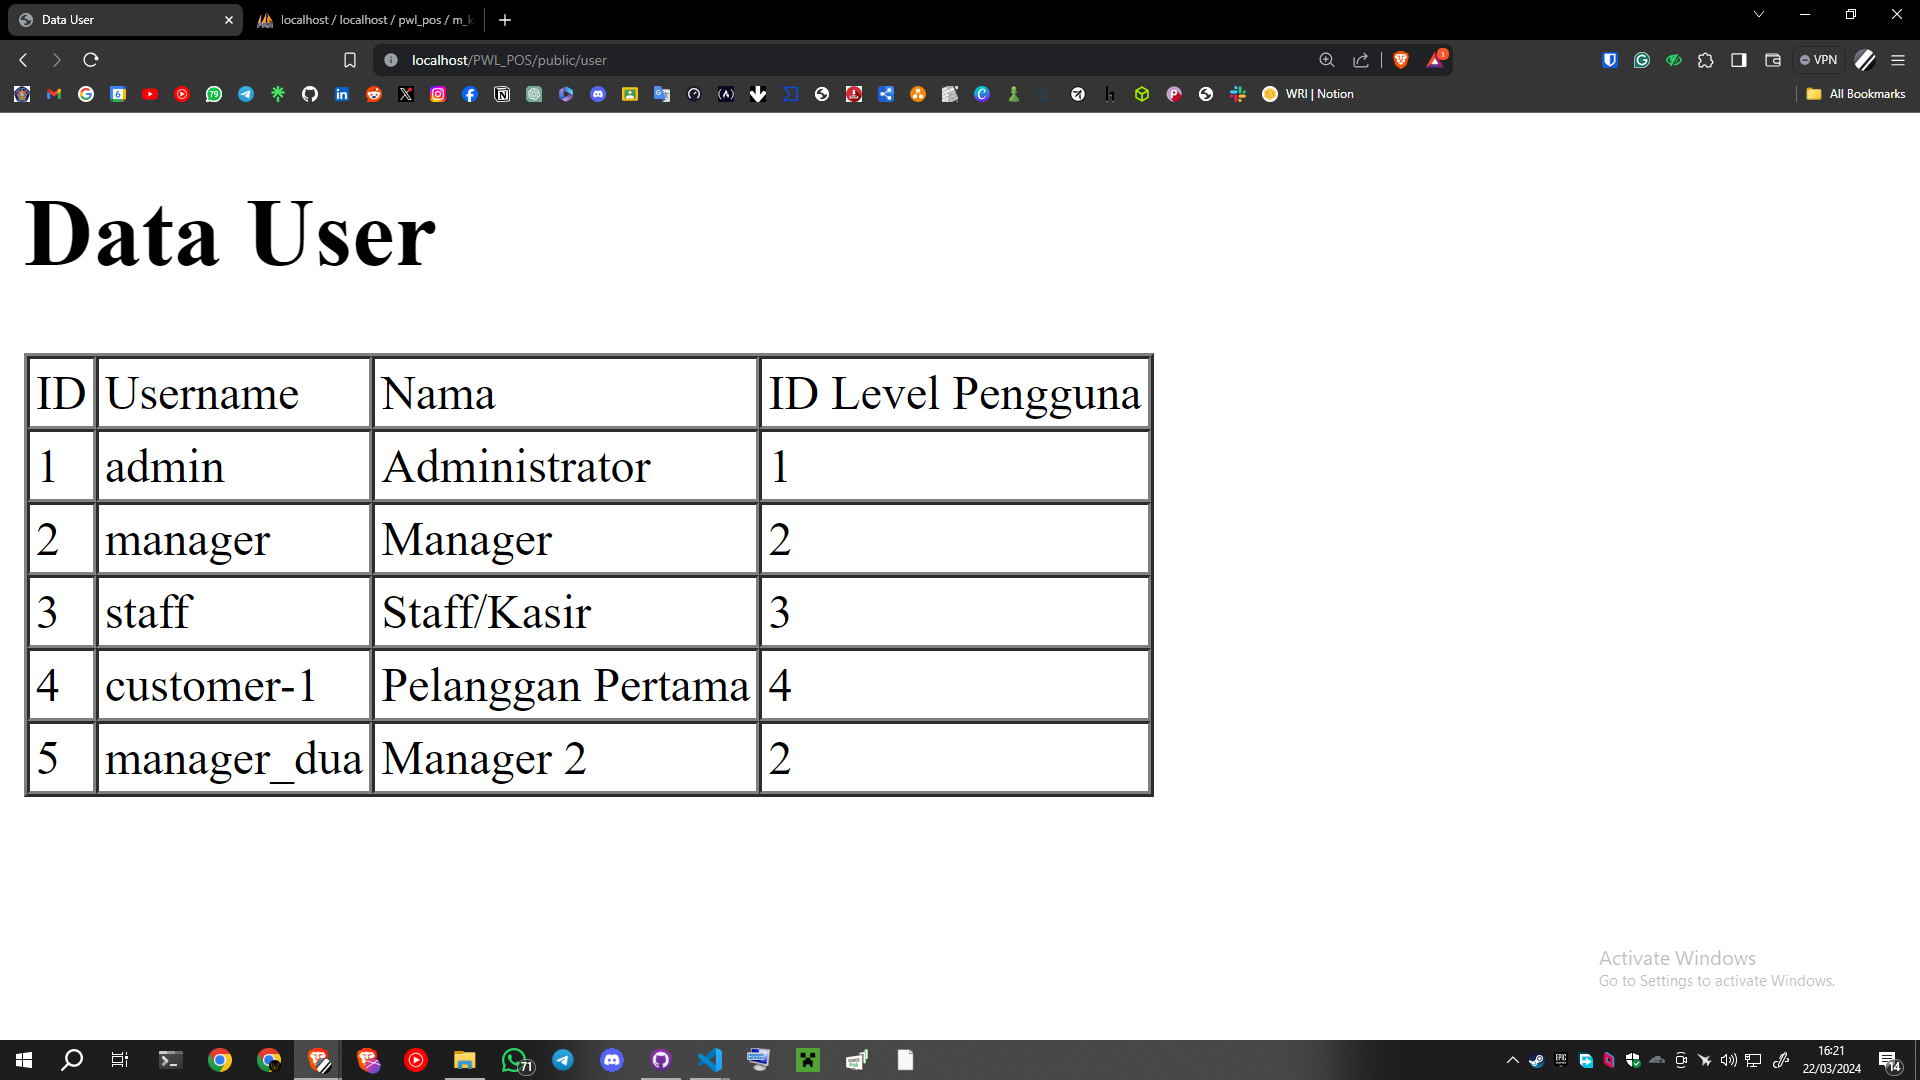
\includegraphics[width=.9\textwidth]{images/figures/Screenshot (395).png} \\ \includegraphics[width=.9\textwidth]{images/figures/Screenshot (396).png} \\ a new user named 'Manager 2' is created
    \newpage
    \item[6.] -  \\ \includegraphics[width=.9\textwidth]{images/figures/Screenshot (397).png} \\ an error occured because 'password' has been removed from fillable. to fix this we need to add 'password' back to the fillable list
\end{enumerate}

\section{Practicum 2.1}
\begin{enumerate}
    \item[3.] - \\ \includegraphics[width=.9\textwidth]{images/figures/Screenshot (398).png} \\ it query the user with id 1
    \item[5.] - \\ 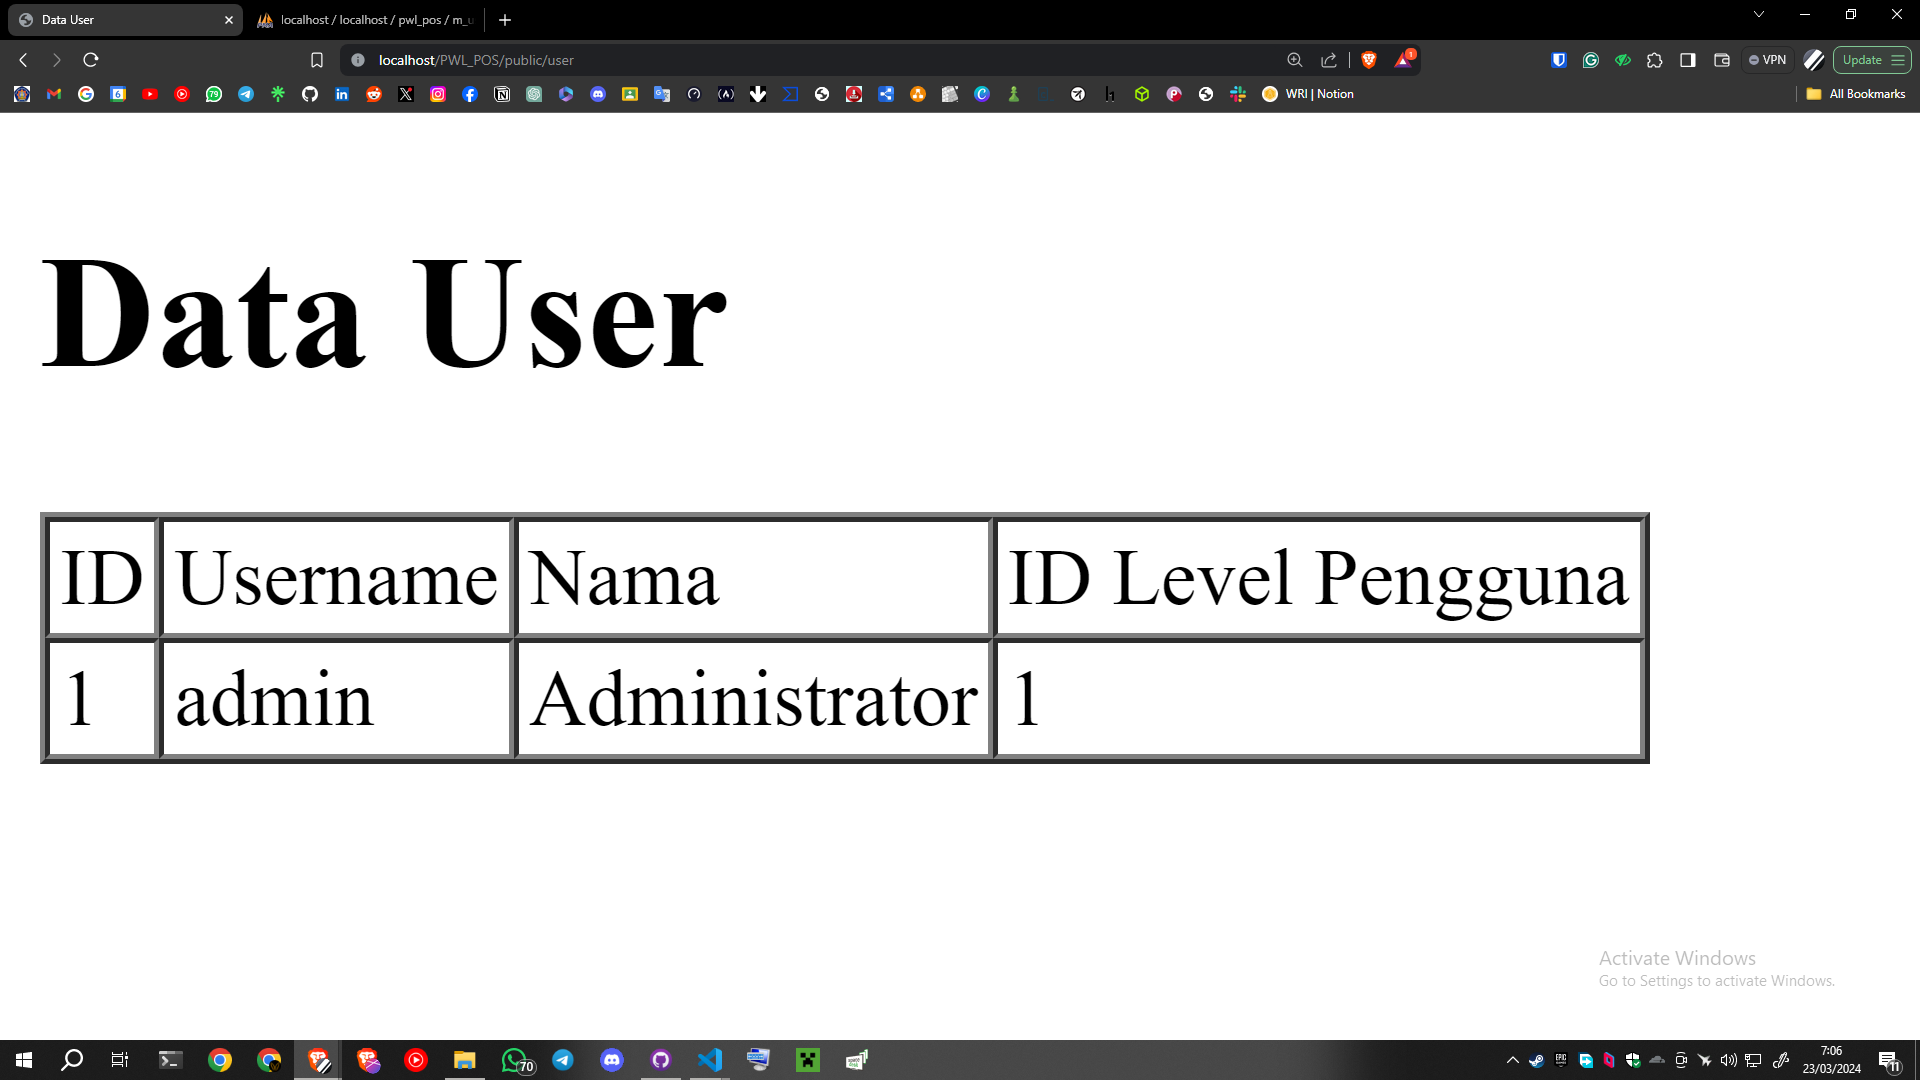
\includegraphics[width=.9\textwidth]{images/figures/Screenshot (399).png} \\ it query the first user in the table with the level\textunderscore id of 1
    \item[7.] - \\ \includegraphics[width=.9\textwidth]{images/figures/Screenshot (400).png} \\ it also query the first user in the table with the level\textunderscore id of 1 with shortcut
    \item[9.] - \\ 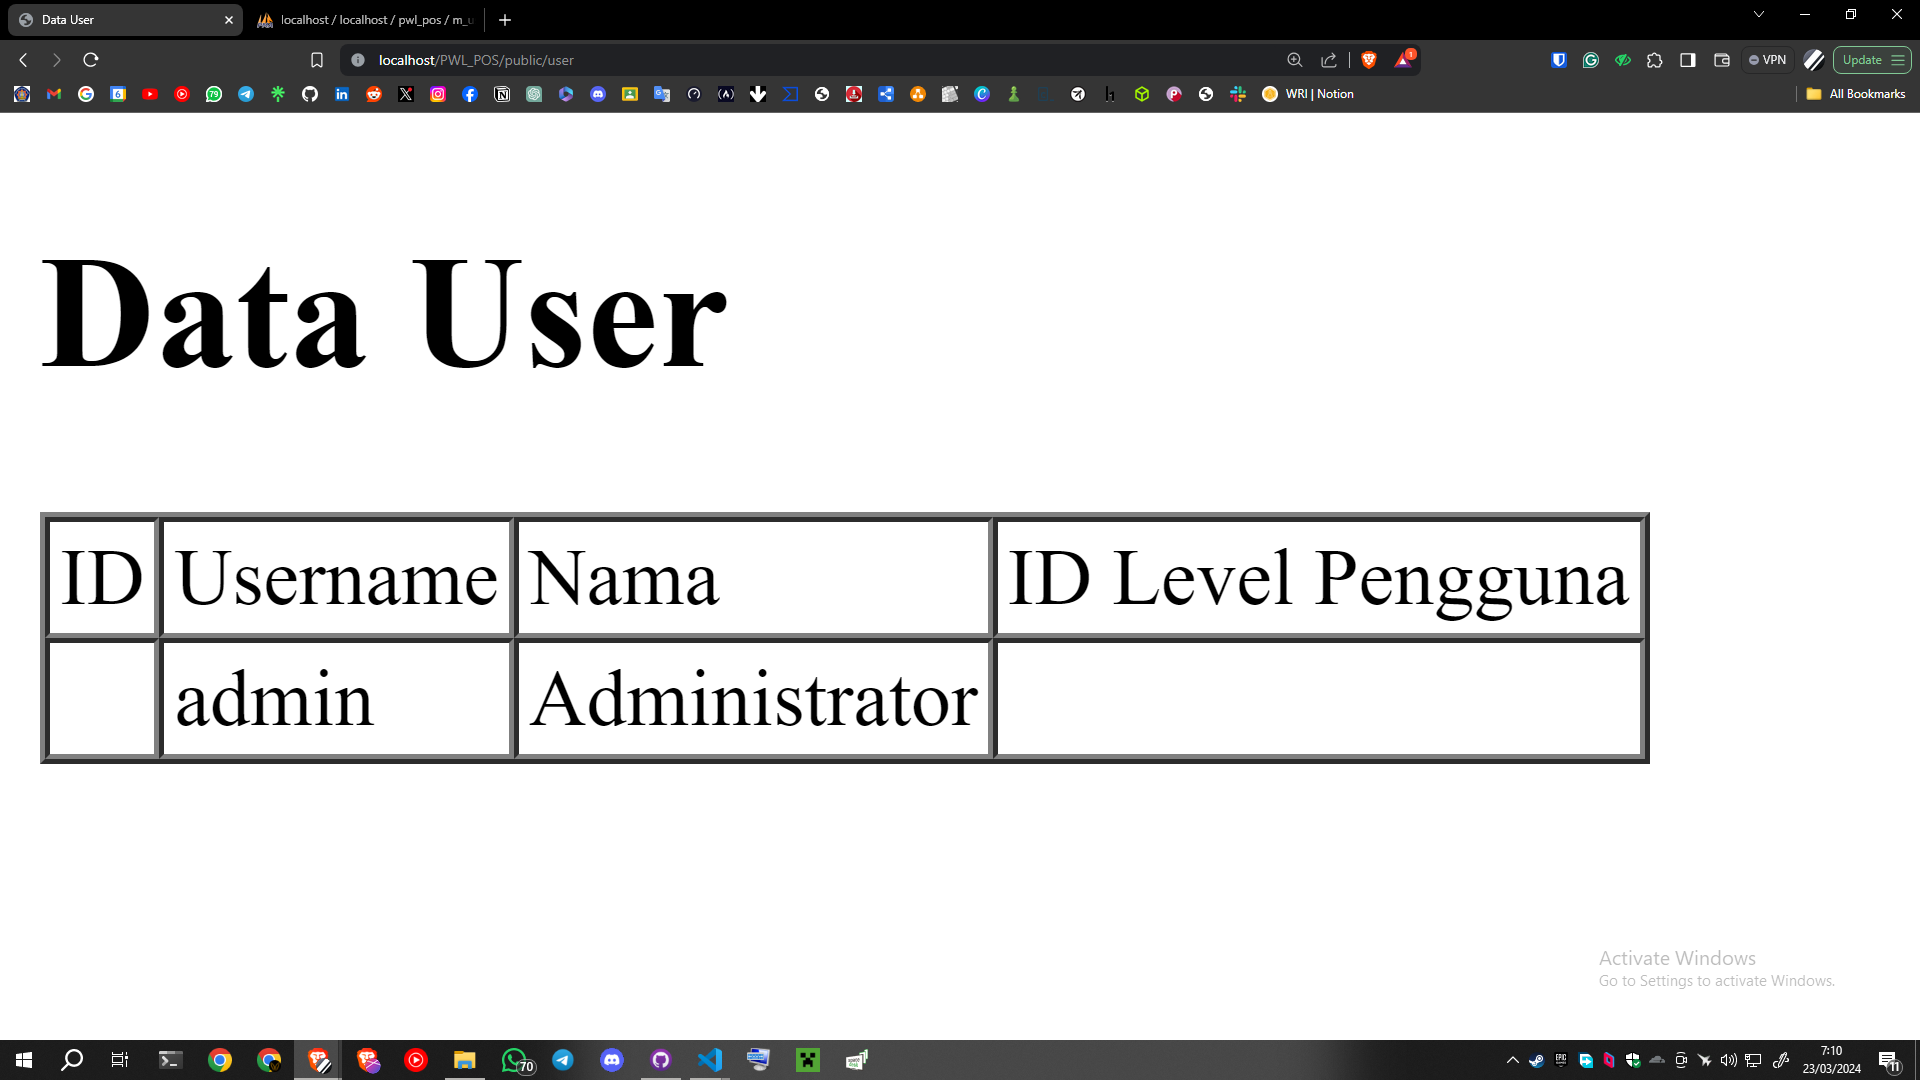
\includegraphics[width=.9\textwidth]{images/figures/Screenshot (401).png} \\ it try query as the parameter dictated, if fails it return as the function inside the parameter dictated
    \item[11.] - \\ \includegraphics[width=.9\textwidth]{images/figures/Screenshot (402).png} \\ it failed query and return an 'abort 404'
\end{enumerate}

\section{Practicum 2.2}
\begin{enumerate}
    \item[2.] - \\ \includegraphics[width=.9\textwidth]{images/figures/Screenshot (403).png} \\ it does the same thing as  Practicum 2.1 step 11 but it is using the shortcut
    \item[4.] - \\ 
\includegraphics[width=.9\textwidth]{images/figures/Screenshot (404).png} \\ it query for user with username 'manager9' with the condition to search the first result otherwise it return 404
\end{enumerate}

\section{Practicum 2.3}
\begin{enumerate}
    \item[2.] - \\ \includegraphics[width=.9\textwidth]{images/figures/Screenshot (405).png} \\ it return the amount of user with level\textunderscore id of 2 using var dump
\end{enumerate}

\section{Practicum 2.4}
\begin{enumerate}
    \item[3.] - \\ 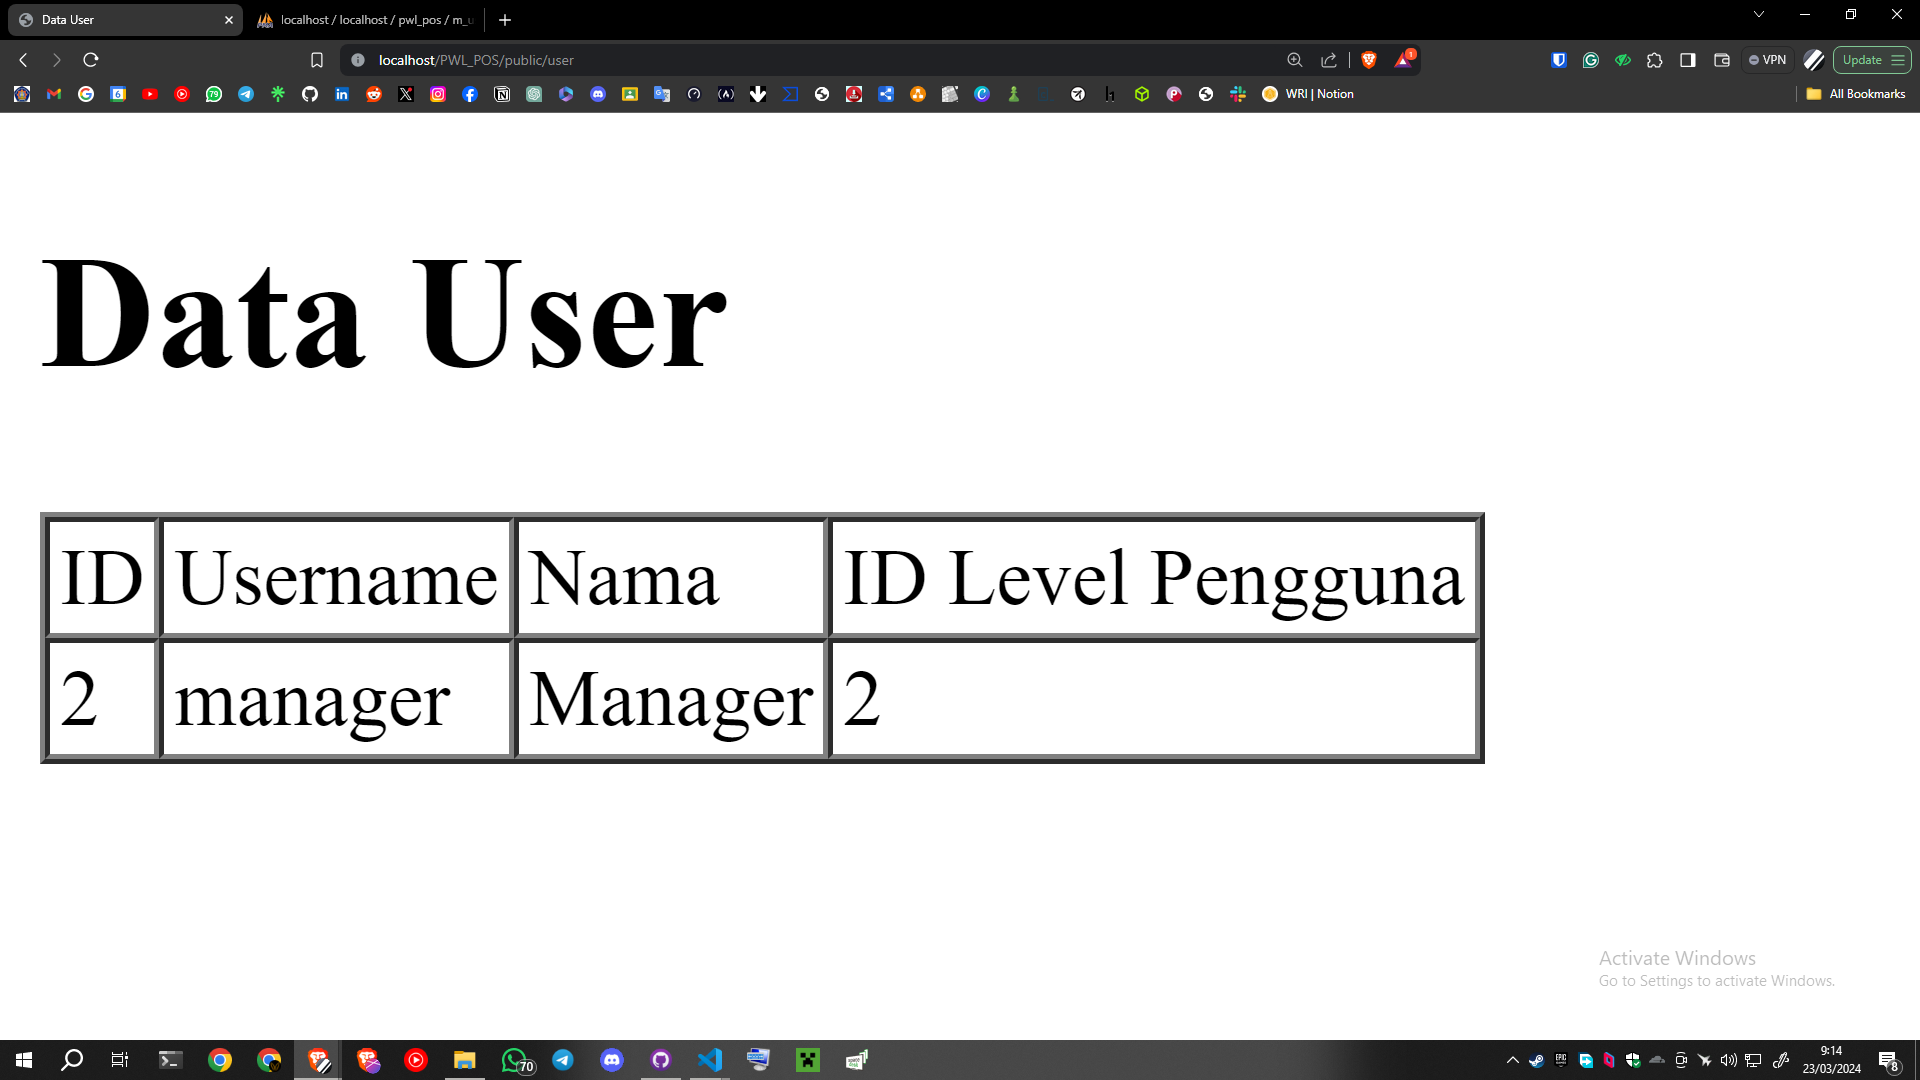
\includegraphics[width=.9\textwidth]{images/figures/Screenshot (407).png} \\ it query the first user with the parameter or create it if it is not yet created
    \item[5.] - \\ 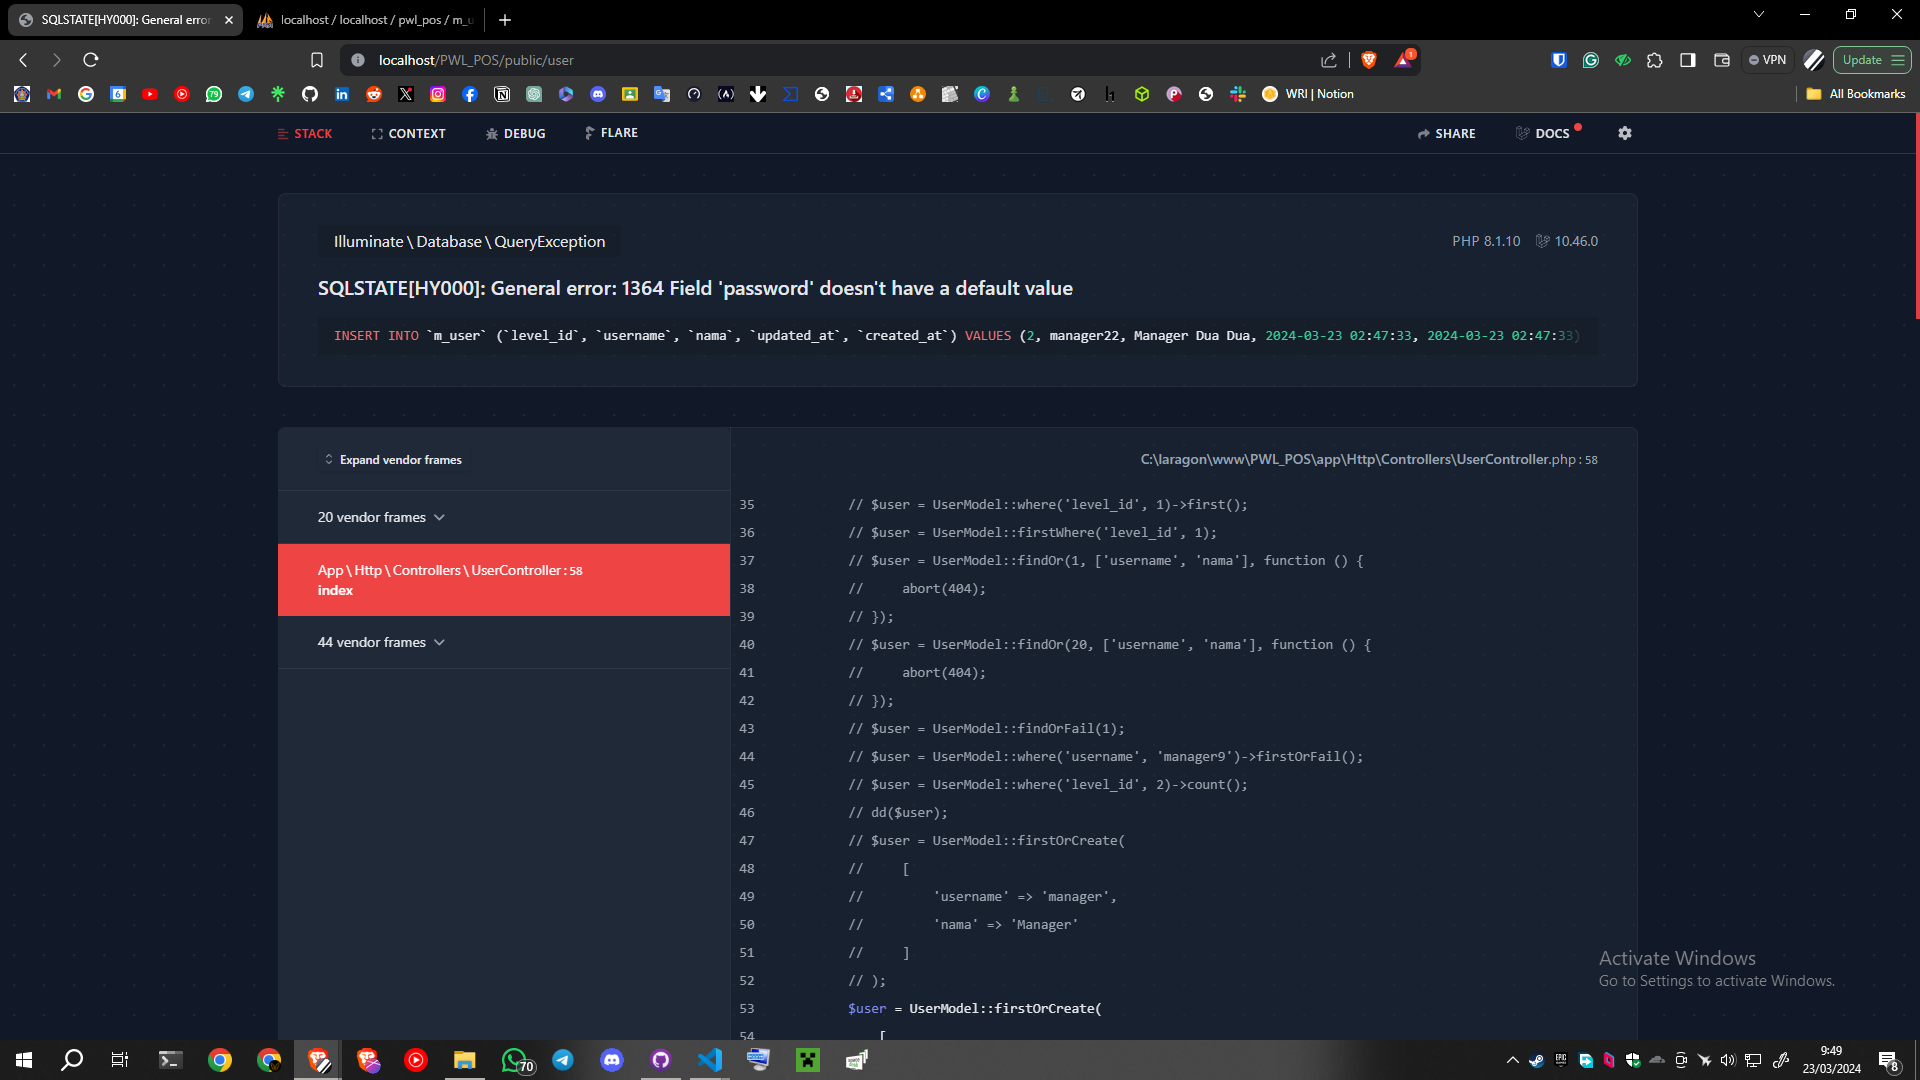
\includegraphics[width=.9\textwidth]{images/figures/Screenshot (408).png} \\ \includegraphics[width=.9\textwidth]{images/figures/Screenshot (409).png} \\ 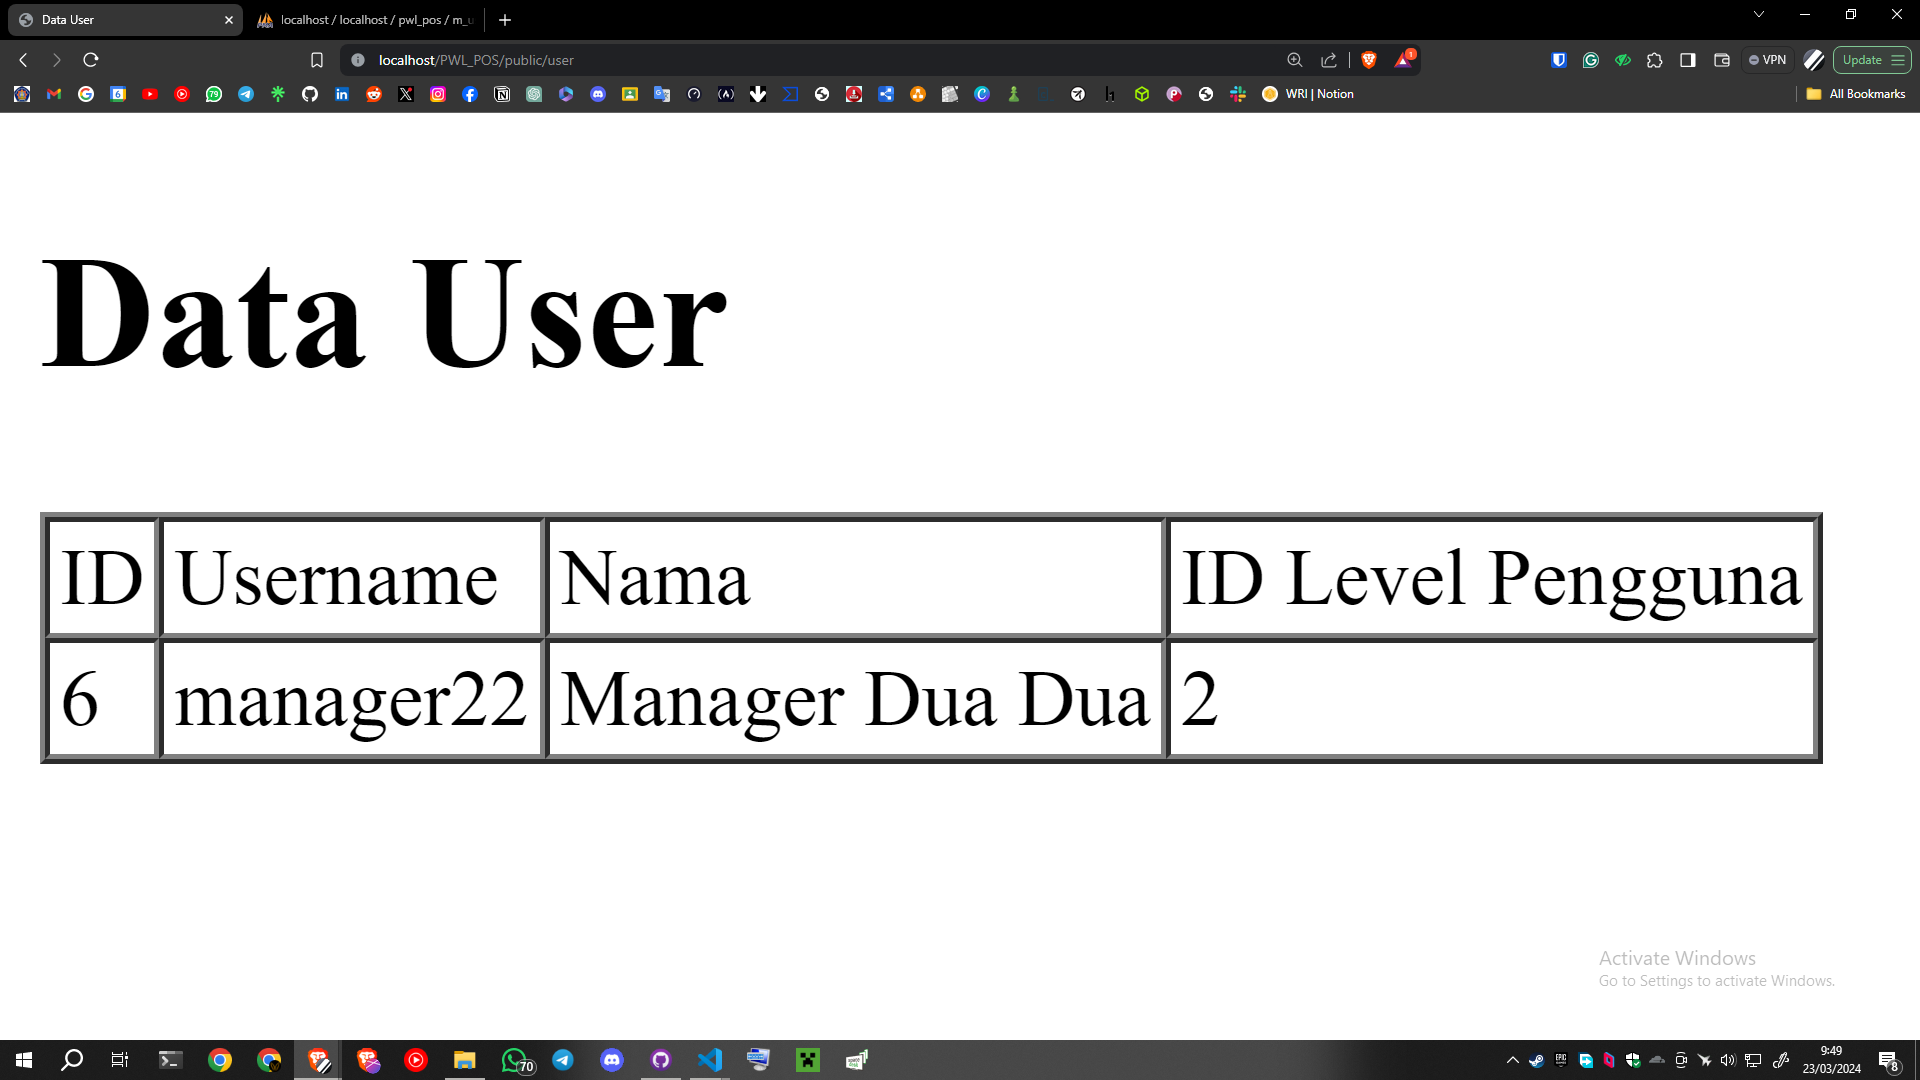
\includegraphics[width=.9\textwidth]{images/figures/Screenshot (410).png} \\ it return an error because previously we havent add 'password' to the fillable. we fixed them and now the user with attribute of the parameter has been created becase user with the attribute of the parameter did not exist before
    \item[7.] - \\ \includegraphics[width=.9\textwidth]{images/figures/Screenshot (412).png} \\ \includegraphics[width=.9\textwidth]{images/figures/Screenshot (411).png} \\ it query the first user that match the parameter
    \item[9.] - \\ \includegraphics[width=.9\textwidth]{images/figures/Screenshot (413).png} \\ 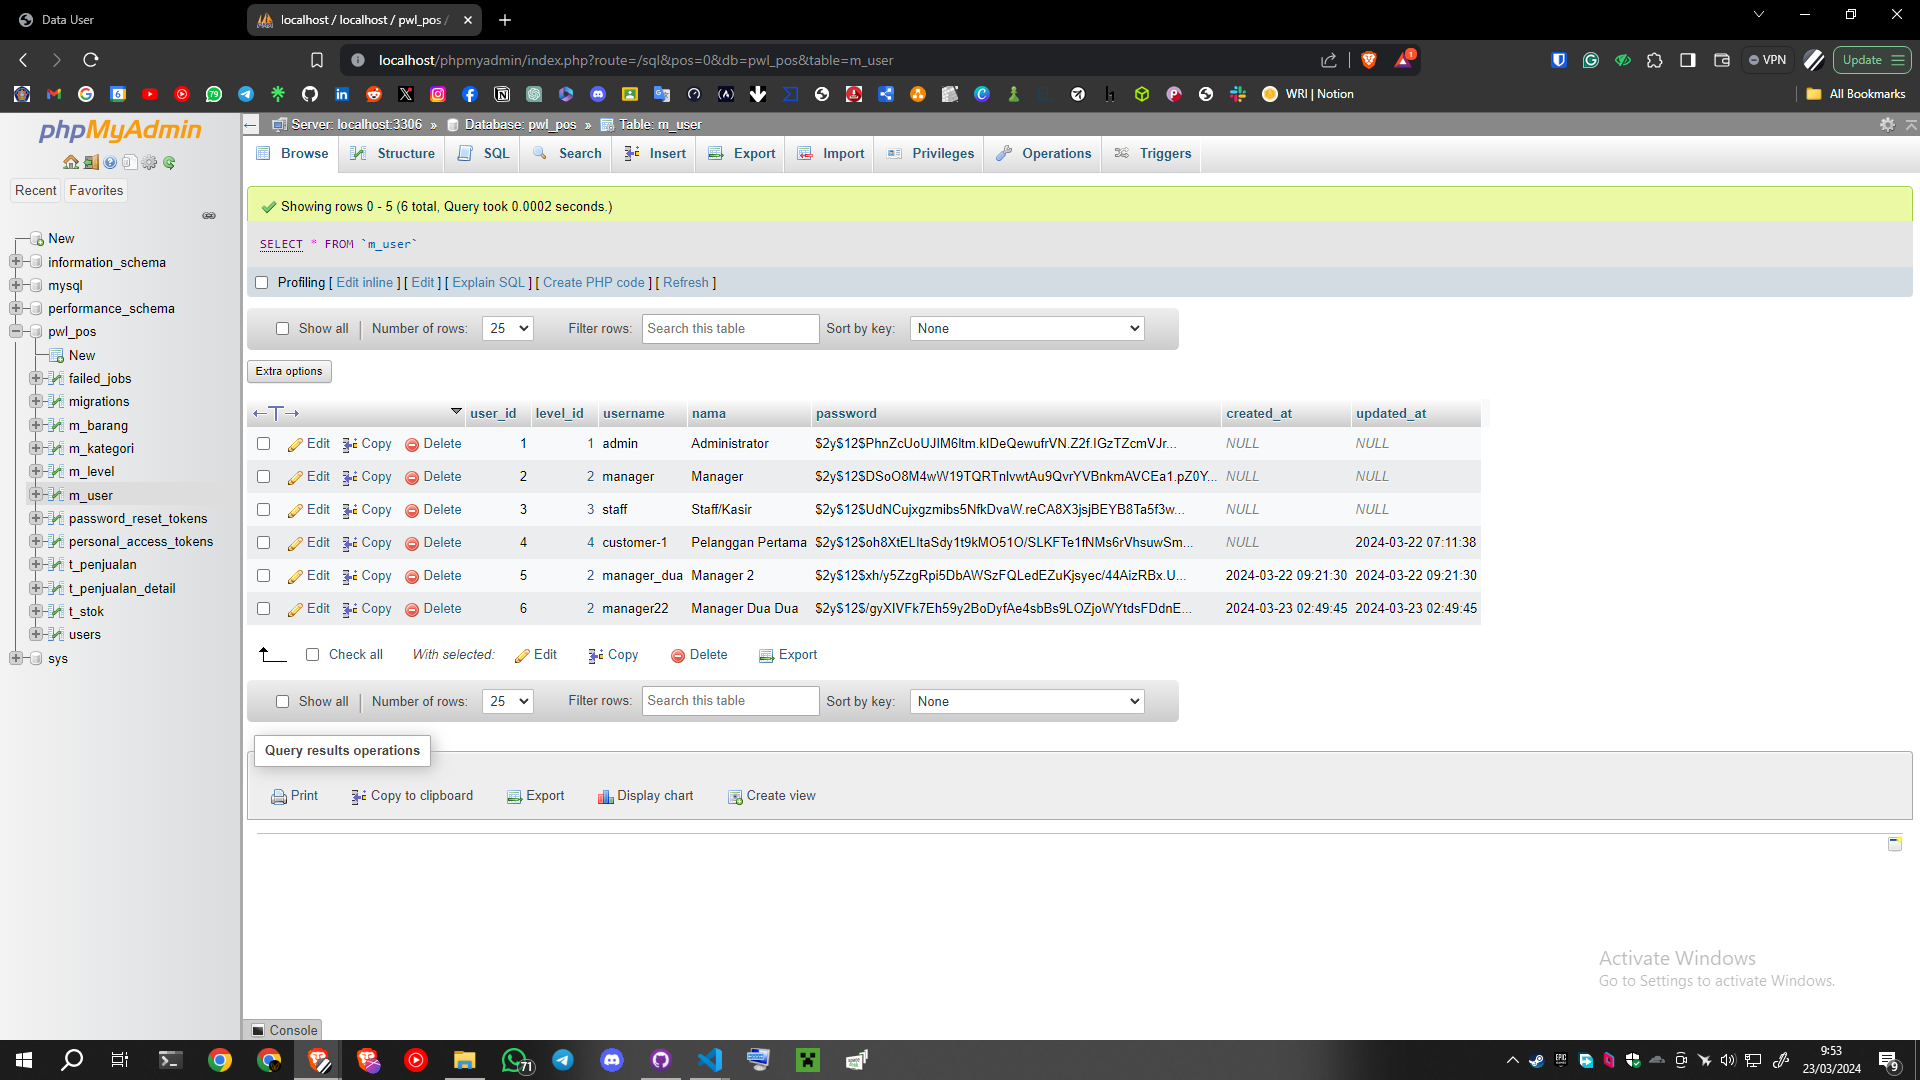
\includegraphics[width=.9\textwidth]{images/figures/Screenshot (414).png} \\ it create an instance of a new user but the data is not presistent to the database
    \item[11.] - \\ \includegraphics[width=.9\textwidth]{images/figures/Screenshot (417).png} \\ 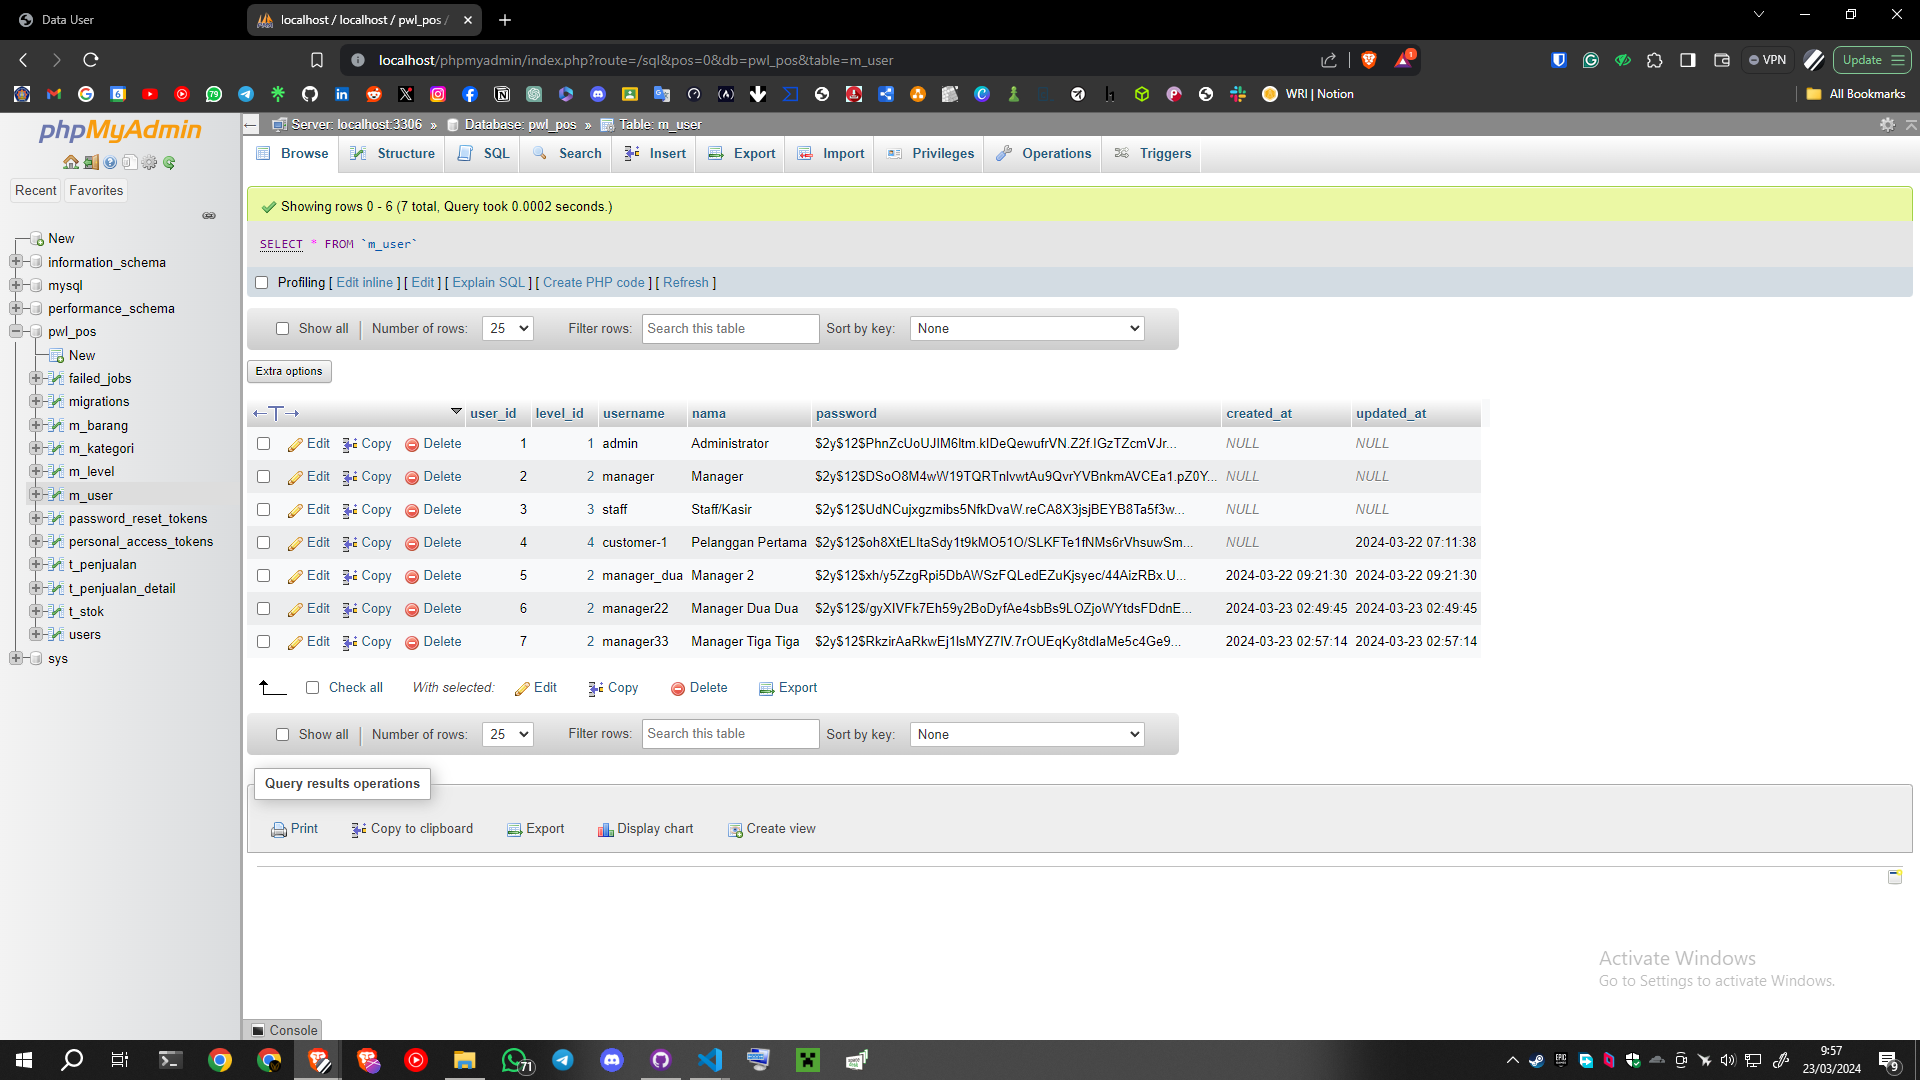
\includegraphics[width=.9\textwidth]{images/figures/Screenshot (418).png} \\ it is now saved to the database
\end{enumerate}

\end{document}